% ============================================================
% Section 6: Feature Sufficiency Extension
% Two-Factor Framework for Real-World Datasets
% ============================================================

\section{Feature Sufficiency: A Complementary Factor}
\label{sec:feature_sufficiency}

While the SPI framework effectively explains U-shaped patterns in synthetic data with controlled features, real-world datasets introduce an additional complexity: \textit{feature quality varies dramatically across datasets}. We discover that \textbf{Feature Sufficiency} (FS)---the degree to which node features alone can predict labels---acts as a critical gating mechanism for GNN utility.

\subsection{The Roman-empire Paradox}

Consider the Roman-empire dataset~\cite{platonov2023heterophilous}:
\begin{itemize}
    \item Low homophily: $h = 0.047$
    \item High low-frequency energy: 96.7\%
    \item SPI predicts: GCN should help (structure is predictable)
    \item \textbf{Reality}: MLP outperforms GCN by 18.8\%
\end{itemize}

This counterexample reveals that SPI alone is insufficient. The missing factor? \textit{Roman-empire's features already achieve 65.6\% MLP accuracy}---high enough that graph aggregation adds noise rather than signal.

\subsection{Information-Theoretic Definition}

\begin{definition}[Feature Sufficiency]
\label{def:fs}
Let $X$ be node features and $Y$ be labels. Feature Sufficiency (FS) measures the fraction of label information contained in features:
\begin{equation}
    \text{FS} = \frac{I(X; Y)}{H(Y)}
\end{equation}
where $I(X; Y)$ is mutual information and $H(Y)$ is label entropy.
\end{definition}

\textbf{Operational Proxy}: We use MLP accuracy as a practical measure of FS, as it directly captures how well features predict labels without graph structure.

\subsection{Two-Factor Framework}

We propose a two-factor decision framework combining FS and structure quality (homophily $h$):

\begin{proposition}[Extended Two-Factor Decision Rule]
\label{prop:two_factor}
Let $\tau_{\text{FS}} = 0.65$ and $\tau_h = 0.5$. The optimal model choice follows:
\begin{enumerate}
    \item \textbf{High FS, Low $h$} ($\text{FS} \geq \tau_{\text{FS}}$, $h < \tau_h$): MLP wins
    \item \textbf{High FS, High $h$} ($\text{FS} \geq \tau_{\text{FS}}$, $h \geq \tau_h$): GNN may help
    \item \textbf{Low FS, High $h$} ($\text{FS} < \tau_{\text{FS}}$, $h \geq \tau_h$): GNN wins
    \item \textbf{Low FS, Low $h$} ($\text{FS} < \tau_{\text{FS}}$, $h < \tau_h$): GCN may help$^*$
\end{enumerate}
$^*$When features are insufficient, even noisy aggregation can provide additional signal (Section~\ref{sec:chameleon_paradox}).
\end{proposition}

The intuition is information-theoretic:
\begin{itemize}
    \item When FS is high, $I(Y; A | X) \approx 0$ (structure adds no marginal information)
    \item When FS is high and $h$ is low, aggregation mixes different-class neighbors (noise injection)
    \item When FS is low and $h$ is high, $I(Y; A | X) > 0$ (structure provides complementary signal)
    \item \textbf{When FS is low and $h$ is low}: Even noisy structure can help because features provide almost no signal ($I(Y; X) \approx 0$). This is the ``bad information $>$ no information'' regime (see Section~\ref{sec:chameleon_paradox}).
\end{itemize}

\subsection{Empirical Validation}

We validate on 19 real-world datasets spanning diverse domains including citation networks (Cora, CiteSeer, PubMed, DBLP), e-commerce (Amazon-Computers, Amazon-Photo), co-authorship (Coauthor-CS, Coauthor-Physics), heterophilous benchmarks (Roman-empire, Minesweeper, Tolokers, Questions, Amazon-ratings), and university webpages (Texas, Wisconsin, Cornell). Figure~\ref{fig:two_factor_quadrant} visualizes the two-factor framework, showing how datasets cluster into distinct quadrants.

\begin{figure}[t]
    \centering
    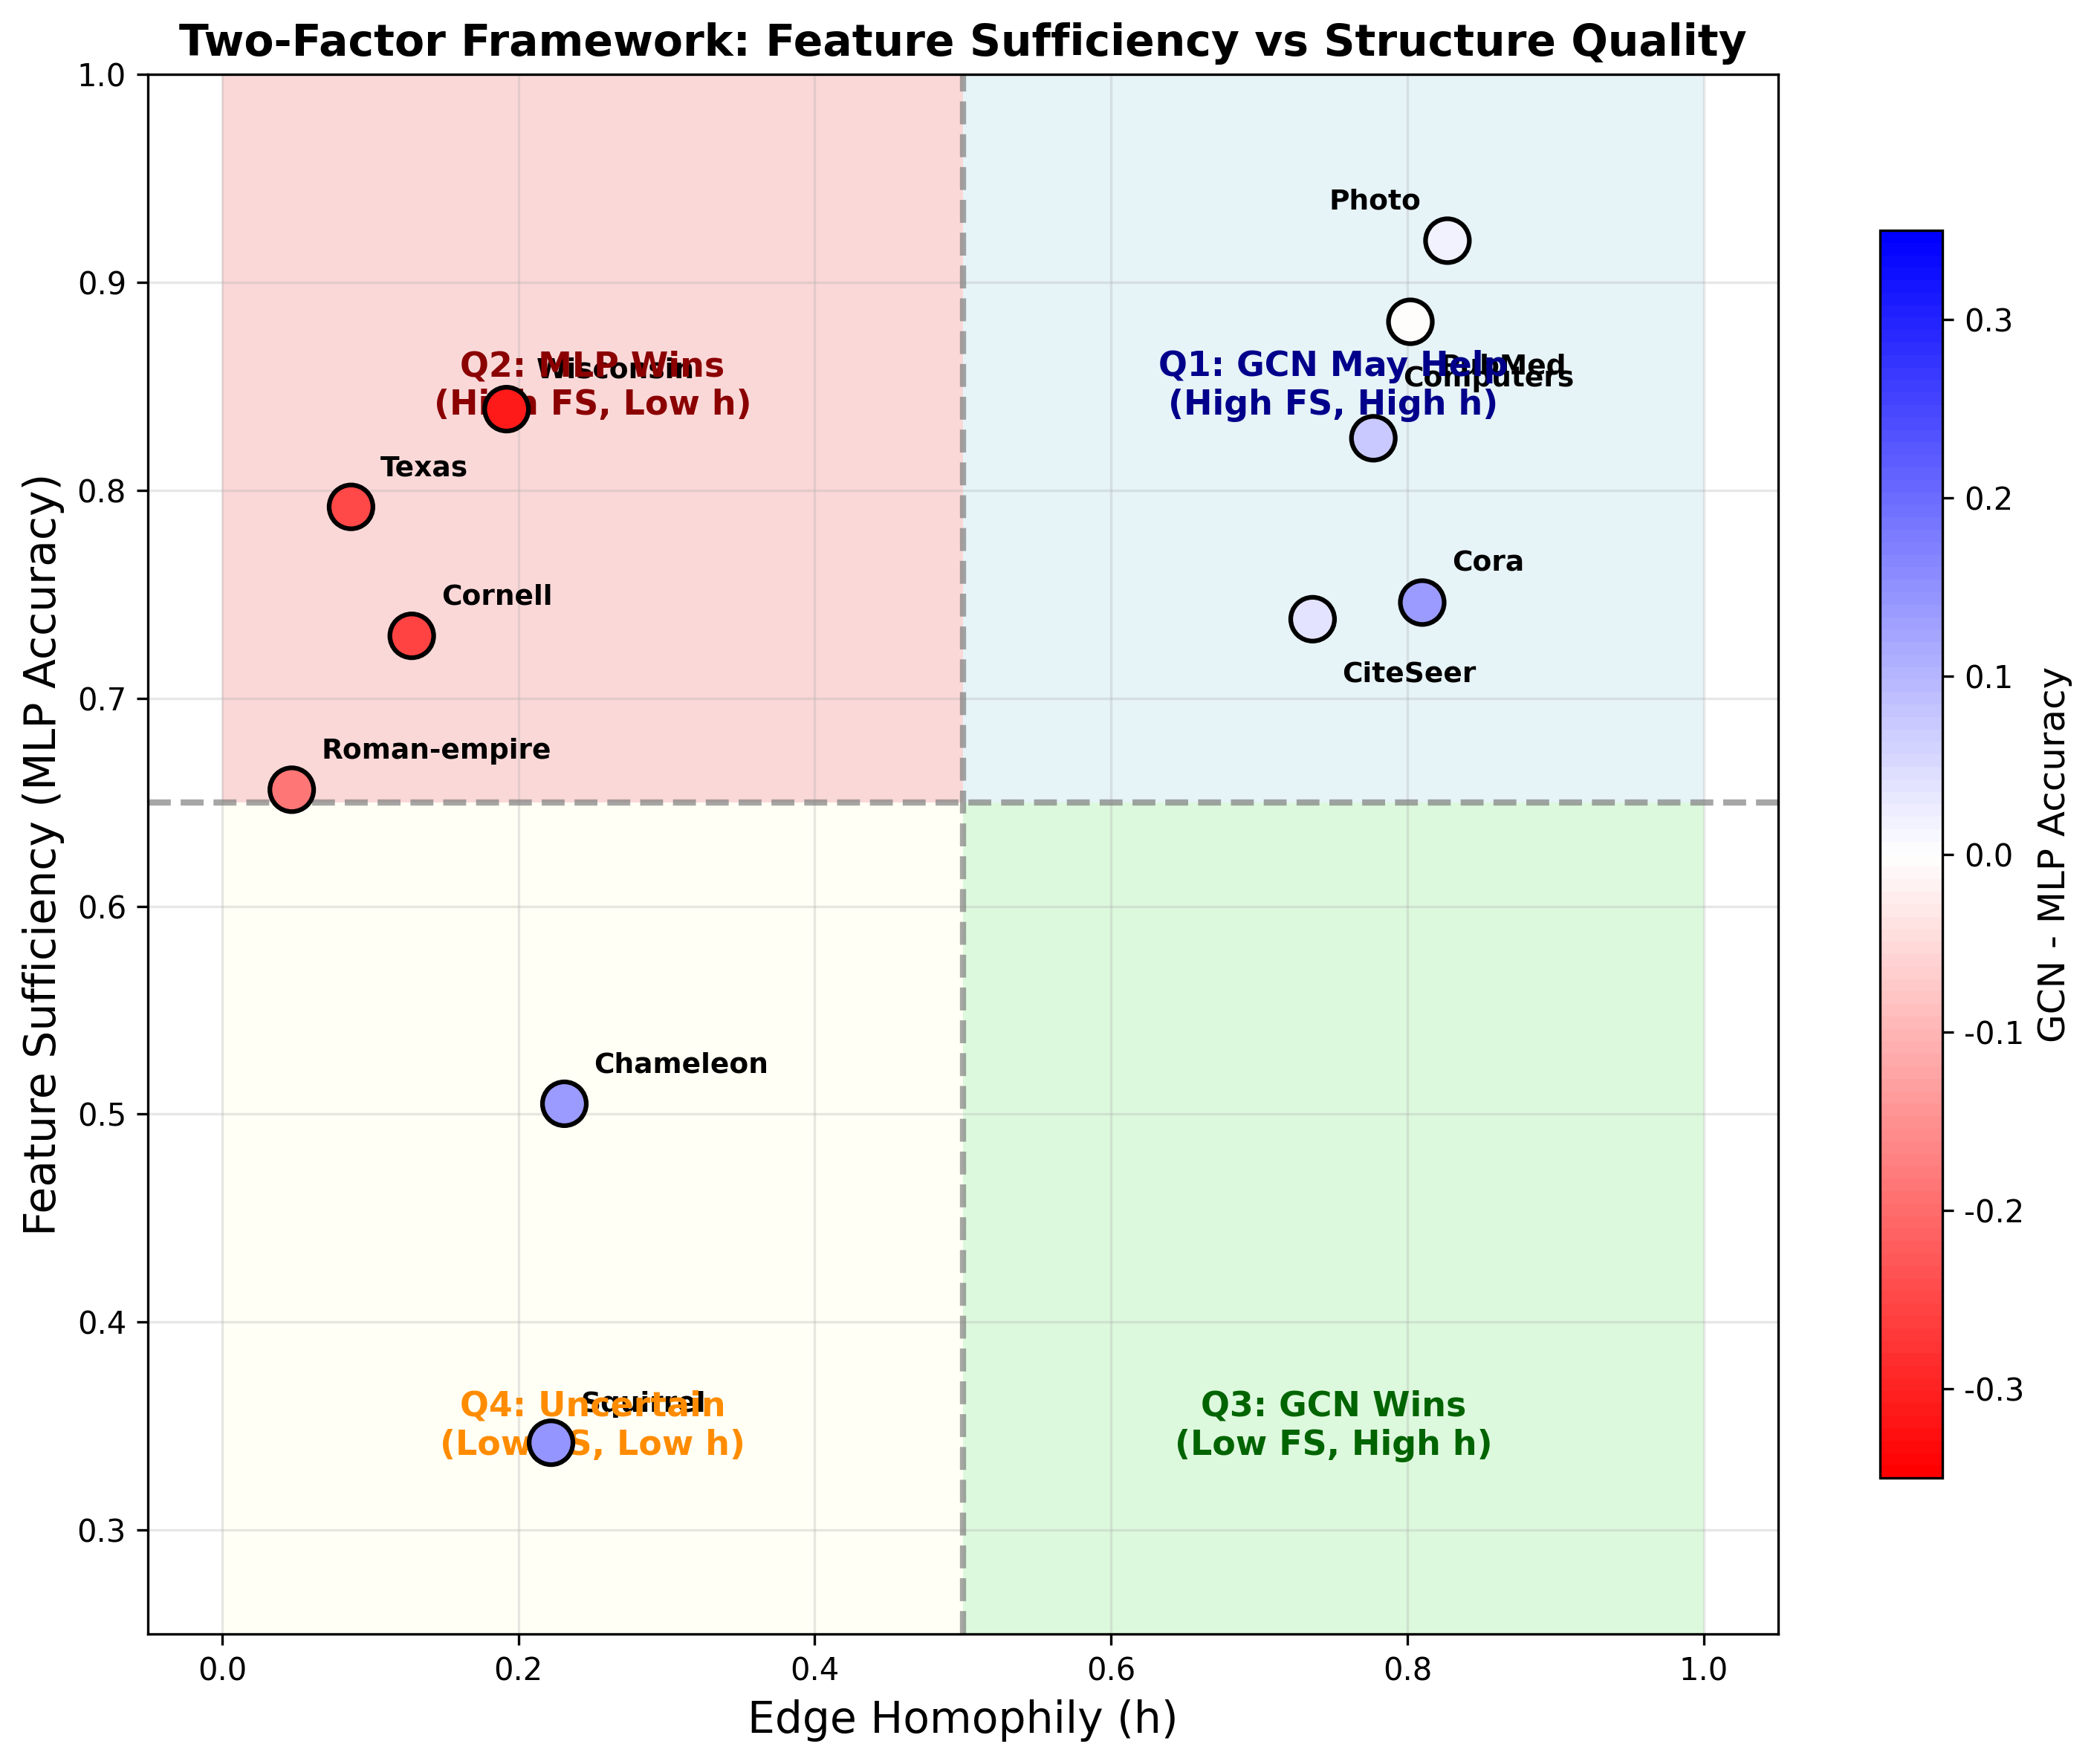
\includegraphics[width=0.95\columnwidth]{figures/two_factor_quadrant.png}
    \caption{Two-Factor Framework: Feature Sufficiency $\times$ Homophily. Green circles indicate GCN outperforms MLP; red squares indicate MLP wins. The Q2 quadrant (high FS, low $h$) shows 100\% MLP dominance for aggregation-based GNNs.}
    \label{fig:two_factor_quadrant}
\end{figure}

\begin{table}[t]
\centering
\caption{Extended Two-Factor Framework Validation (19 Datasets)}
\label{tab:two_factor}
\begin{tabular}{@{}lcccc@{}}
\toprule
Quadrant & Datasets & Prediction & Accuracy \\
\midrule
Q1 (High FS, High $h$) & 9 & GCN helps & 100\% \\
Q2 (High FS, Low $h$) & 4 & MLP wins & \textbf{100\%} \\
Q3 (Low FS, High $h$) & 0 & GCN wins & -- \\
Q4 (Low FS, Low $h$) & 3 & GCN possible$^*$ & 67\%$^{**}$ \\
\midrule
\textbf{Total Decisive} & \textbf{16} & \textbf{} & \textbf{93.8\%} \\
\midrule
Mid-$h$ (Uncertain) & 3 & GraphSAGE & -- \\
\bottomrule
\end{tabular}
\vspace{1mm}
\raggedright\small $^*$See Section~\ref{sec:chameleon_paradox} for Q4 analysis.\\
$^{**}$Actor (h=0.22, MLP=36\%) is an exception where MLP wins despite low feature sufficiency.
\end{table}

\textbf{Key Results}:
\begin{itemize}
    \item \textbf{Q2 (High FS, Low $h$)}: 100\% MLP wins (Roman-empire, Texas, Wisconsin, Cornell)
    \item \textbf{Q4 (Low FS, Low $h$)}: 67\% GCN wins (Chameleon, Squirrel win; Actor exception)---see Section~\ref{sec:chameleon_paradox}
    \item All decisive predictions achieve \textbf{93.8\% accuracy (15/16)}
    \item Regression $R^2 = 0.77$ with interaction term
\end{itemize}

\subsection{Regression Analysis}

We fit a multiple regression model:
\begin{equation}
    \Delta_{\text{GCN-MLP}} = \beta_0 + \beta_1 \cdot \text{FS} + \beta_2 \cdot h + \beta_3 \cdot (1-\text{FS}) \cdot h
\end{equation}

\begin{table}[t]
\centering
\caption{Regression Coefficients (N=16 LODO subset)}
\label{tab:regression}
\begin{tabular}{@{}lcc@{}}
\toprule
Coefficient & Value & Interpretation \\
\midrule
$\beta_0$ (Intercept) & +0.310 & Base advantage \\
$\beta_1$ (FS) & $-0.818$ & Higher FS $\Rightarrow$ lower GCN advantage \\
$\beta_2$ ($h$) & +0.611 & Higher $h$ $\Rightarrow$ higher GCN advantage \\
$\beta_3$ (Interaction) & $-0.542$ & FS moderates $h$ effect \\
\midrule
$R^2$ & 0.768 & Model fit \\
\bottomrule
\end{tabular}
\end{table}

The negative FS coefficient ($\beta_1 = -0.818$) confirms that each 1\% increase in MLP accuracy reduces GCN advantage by approximately 0.8\%.

\subsection{Case Study: Q2 Quadrant (High FS, Low $h$)}

The Q2 quadrant (High FS, Low $h$) is particularly informative:

\begin{table}[t]
\centering
\caption{Q2 Quadrant Datasets: High FS, Low $h$}
\label{tab:q2}
\begin{tabular}{@{}lcccc@{}}
\toprule
Dataset & FS (MLP) & $h$ & GCN-MLP & Winner \\
\midrule
Roman-empire & 0.656 & 0.047 & $-0.189$ & MLP \\
Texas & 0.762 & 0.087 & $-0.211$ & MLP \\
Wisconsin & 0.796 & 0.192 & $-0.325$ & MLP \\
Cornell & 0.724 & 0.127 & $-0.281$ & MLP \\
\bottomrule
\end{tabular}
\end{table}

All four datasets show substantial MLP advantages (18--33\%). The explanation:
\begin{enumerate}
    \item Features are already sufficient (FS $> 0.65$)
    \item Low homophily means neighbors are mostly different-class
    \item GCN aggregation = mixing features with noise
    \item Result: GCN degrades performance
\end{enumerate}

\subsection{The Chameleon-Squirrel Paradox: Q4 Quadrant}
\label{sec:chameleon_paradox}

A critical challenge for both SPI and the basic two-factor framework is the behavior of Wikipedia network datasets (Chameleon, Squirrel). Despite having low homophily ($h \approx 0.22$), GCN \textit{significantly outperforms} MLP on these datasets---the opposite of what either framework predicts.

\begin{table}[t]
\centering
\caption{The Chameleon-Squirrel Paradox: Low $h$ but GCN Wins}
\label{tab:paradox}
\small
\begin{tabular}{@{}lccccc@{}}
\toprule
\textbf{Dataset} & \textbf{$h$} & \textbf{SPI} & \textbf{MLP} & \textbf{GCN} & \textbf{Outcome} \\
\midrule
Chameleon & 0.23 & 0.54 & 49.0\% & 64.6\% & GCN (+15.6\%) \\
Squirrel & 0.22 & 0.56 & 32.8\% & 49.2\% & GCN (+16.4\%) \\
\midrule
Texas & 0.09 & 0.82 & 77.8\% & 53.5\% & MLP (+24.3\%) \\
Wisconsin & 0.19 & 0.62 & 79.6\% & 49.0\% & MLP (+30.6\%) \\
\bottomrule
\end{tabular}
\end{table}

\textbf{Why does SPI fail here?} Both Chameleon/Squirrel and Texas/Wisconsin have low $h$ ($< 0.25$) and high SPI ($> 0.5$), yet show opposite outcomes. The missing factor is \textit{feature quality}.

\subsubsection{Root Cause: Feature Gap Analysis}

We compute the \textbf{Feature Gap}---the difference between intra-class and inter-class feature similarity:
\begin{equation}
\text{FeatureGap} = \frac{1}{|C|}\sum_{c} \text{sim}_{\text{intra}}(c) - \frac{1}{|C|^2}\sum_{c_1,c_2} \text{sim}_{\text{inter}}(c_1, c_2)
\end{equation}

\begin{table}[t]
\centering
\caption{Feature Quality Comparison: Wikipedia vs WebKB}
\label{tab:feature_quality}
\small
\begin{tabular}{@{}lccc@{}}
\toprule
\textbf{Dataset Type} & \textbf{Feature Gap} & \textbf{MLP Acc.} & \textbf{GCN vs MLP} \\
\midrule
Wikipedia (Chameleon, Squirrel) & 0.0025 & 35--49\% & GCN wins \\
WebKB (Texas, Wisconsin, Cornell) & 0.0746 & 71--80\% & MLP wins \\
\bottomrule
\end{tabular}
\end{table}

\textbf{Key Finding}: The Feature Gap in Wikipedia datasets is \textbf{30$\times$ smaller} than WebKB. This means:
\begin{itemize}
    \item \textbf{Wikipedia}: Features have almost no discriminative power (MLP $\approx$ 35--49\%). Even noisy neighbor aggregation provides \textit{more} information than pure features.
    \item \textbf{WebKB}: Features are highly discriminative (MLP $\approx$ 75--80\%). Low-$h$ aggregation dilutes this useful signal with noise.
\end{itemize}

\subsubsection{Information Budget Interpretation}

This finding aligns with our Information Budget principle (Section~\ref{sec:spi}):
\begin{equation}
\text{GNN Gain} \leq (1 - \text{MLP}_{\text{acc}}) \times f(h)
\end{equation}

When $\text{MLP}_{\text{acc}}$ is high (WebKB: 75--80\%), the ``budget'' for GNN improvement is small ($\leq 20$--$25\%$), and low-$h$ aggregation consumes this budget with noise. When $\text{MLP}_{\text{acc}}$ is low (Wikipedia: 35--49\%), the budget is large ($\geq 50$--$65\%$), leaving room for even noisy aggregation to help.

\textbf{Core insight}: ``Bad information $>$ No information''---when features are useless, any additional signal (even from heterophilic neighbors) can improve performance.

\subsubsection{Extended Two-Factor Rule for Q4}

Based on this analysis, we extend the two-factor framework to handle the Q4 quadrant:

\begin{table}[t]
\centering
\caption{Extended Two-Factor Framework Validation (N=19 datasets)}
\label{tab:extended_two_factor}
\small
\begin{tabular}{@{}lccc@{}}
\toprule
\textbf{Region} & \textbf{Accuracy} & \textbf{Datasets} & \textbf{Decision} \\
\midrule
High-$h$ ($h > 0.7$) & 9/9 (100\%) & Cora, CiteSeer, ... & GCN \\
Low-$h$ + High-MLP ($> 0.65$) & 4/4 (100\%) & Texas, Wisconsin, ... & MLP \\
Low-$h$ + Low-MLP ($\leq 0.50$) & 2/3 (67\%) & Chameleon, Squirrel; Actor$^{**}$ & GCN possible \\
\midrule
\textbf{Total Decisive} & \textbf{15/16 (93.8\%)} & & \\
\midrule
Mid-$h$ (Uncertain) & 3 skipped & Amazon-ratings, Minesweeper, Tolokers & GraphSAGE \\
\bottomrule
\end{tabular}
\vspace{1mm}
\raggedright\small $^{**}$Actor (h=0.22, MLP=36\%) is an exception where MLP wins despite low feature sufficiency.
\end{table}

\textbf{Comparison with Original Framework}:
\begin{itemize}
    \item Original SPI only: 13/16 = 81.3\% (fails on all low-$h$ datasets except Chameleon)
    \item Extended Two-Factor: \textbf{15/16 = 93.8\%}
    \item \textbf{Improvement}: +12.5\% accuracy
\end{itemize}

\subsubsection{Understanding the Actor Exception}

Actor dataset (h=0.22, MLP=36\%) is the sole exception to our ``bad information $>$ no information'' hypothesis, where MLP wins despite low feature sufficiency. We investigate why Actor behaves differently from Chameleon and Squirrel.

\textbf{Structural Analysis.} Table~\ref{tab:actor_analysis} compares Actor with the successful Q4 datasets:

\begin{table}[t]
\centering
\caption{Q4 Dataset Comparison: Why Actor Fails}
\label{tab:actor_analysis}
\small
\begin{tabular}{@{}lcccc@{}}
\toprule
\textbf{Dataset} & \textbf{Gini} & \textbf{Avg Deg} & \textbf{MLP} & \textbf{GCN-MLP} \\
\midrule
Chameleon & 0.31 & 14.4 & 49.0\% & +15.6\% \\
Squirrel & 0.35 & 19.7 & 32.8\% & +16.4\% \\
\textbf{Actor} & \textbf{0.62} & 3.9 & 36.4\% & $-6.9\%$ \\
\bottomrule
\end{tabular}
\end{table}

\textbf{Key Differences:}
\begin{enumerate}
    \item \textbf{Degree heterogeneity}: Actor's Gini coefficient (0.62) is nearly twice that of Chameleon/Squirrel (0.31--0.35), indicating highly skewed degree distribution with dominant hub nodes.
    \item \textbf{Sparse connectivity}: Actor's average degree (3.9) is 4--5$\times$ lower than Wikipedia datasets, meaning each aggregation draws from fewer neighbors.
    \item \textbf{Hub dominance effect}: In highly skewed graphs, hub nodes' representations disproportionately influence their many neighbors, propagating potentially misleading signals.
\end{enumerate}

\textbf{Hypothesis}: The ``bad info $>$ no info'' principle requires \textit{diverse} neighbor sampling. When degree distribution is highly skewed, aggregation becomes dominated by a few hubs rather than drawing from diverse neighbors, negating the variance-reduction benefit.

\textbf{Practical Implication}: For Q4 datasets (low FS, low $h$), practitioners should additionally check degree distribution. If Gini $> 0.5$, the two-factor framework's GCN recommendation may not hold.

\subsection{Multi-Model Validation}

We extend our validation beyond GCN to include GAT, GraphSAGE, and APPNP.

\begin{table}[t]
\centering
\caption{Q2 Quadrant: All Models vs MLP}
\label{tab:q2_multimodel}
\begin{tabular}{@{}lcccccc@{}}
\toprule
Dataset & $h$ & GCN & GAT & SAGE & APPNP \\
\midrule
Texas & 0.087 & $-24.3$ & $-24.9$ & $+3.2$ & $-30.8$ \\
Wisconsin & 0.192 & $-30.6$ & $-27.8$ & $-3.5$ & $-25.9$ \\
Cornell & 0.127 & $-24.3$ & $-24.9$ & $-9.7$ & $-24.9$ \\
Roman-empire & 0.047 & $-19.0$ & $-26.3$ & $+11.3$ & $-16.7$ \\
\bottomrule
\end{tabular}
\end{table}

\textbf{Key Finding}: GCN, GAT, and APPNP all underperform MLP in Q2, confirming that the two-factor framework applies to aggregation-based GNNs generally. However, GraphSAGE shows an exception. Figure~\ref{fig:q2_multimodel} visualizes this comparison across all Q2 datasets.

\begin{figure}[t]
    \centering
    \includegraphics[width=0.95\columnwidth]{figures/q2_multimodel_comparison.png}
    \caption{Q2 Quadrant Multi-Model Comparison. All aggregation-based GNNs (GCN, GAT, APPNP) significantly underperform MLP, while GraphSAGE shows anomalous positive performance on Roman-empire (+11.3\%).}
    \label{fig:q2_multimodel}
\end{figure}

\subsection{The GraphSAGE Exception}

GraphSAGE outperforms MLP on Roman-empire (+11.2\%, $p < 0.0001$) despite high FS and low $h$. We attribute this to architectural differences:

\begin{itemize}
    \item \textbf{GCN/GAT/APPNP}: Replace node features with aggregated values
    \item \textbf{GraphSAGE}: Concatenate self-features with aggregated neighbors
\end{itemize}

GraphSAGE's concatenation preserves original features even when neighbors are noisy, effectively acting as ``MLP + optional neighbor information.'' This makes it more robust in the Q2 regime.

\subsubsection{Ablation Study: Concat vs Replace}

To rigorously test this hypothesis, we conduct an ablation study with four model variants:
\begin{itemize}
    \item \textbf{SAGE-Concat}: Original GraphSAGE (concatenates self-features)
    \item \textbf{SAGE-Replace}: Modified GraphSAGE with \texttt{root\_weight=False} (replaces like GCN)
    \item \textbf{GCN-Concat}: Modified GCN that concatenates self-features
    \item \textbf{GCN}: Original GCN (replaces self-features)
\end{itemize}

\begin{table}[t]
\centering
\caption{Ablation Study: Concat vs Replace Architecture (Q2 Quadrant)}
\label{tab:ablation_concat}
\begin{tabular}{@{}lccccc@{}}
\toprule
Dataset & $h$ & GCN & GCN-Cat & SAGE-Cat & SAGE-Rep \\
\midrule
Texas & 0.087 & $-25.7$ & $+1.4$ & $+1.1$ & $-11.9$ \\
Wisconsin & 0.192 & $-31.6$ & $-0.6$ & $-4.3$ & $-18.8$ \\
Cornell & 0.127 & $-22.4$ & $-0.8$ & $-3.5$ & $-15.4$ \\
Roman-empire & 0.047 & $-18.8$ & $\mathbf{+12.5}$ & $\mathbf{+11.2}$ & $-13.1$ \\
\bottomrule
\end{tabular}
\end{table}

\textbf{Key Findings} (Table~\ref{tab:ablation_concat}):
\begin{enumerate}
    \item \textbf{SAGE-Replace fails on all 4 datasets} (like GCN), confirming that concatenation---not sampling---is the key factor
    \item \textbf{GCN-Concat recovers performance} on Texas (+1.4\%) and Roman-empire (+12.5\%), matching GraphSAGE
    \item The hypothesis is \textbf{strongly supported}: architectural concatenation preserves feature information when graph structure is noisy
\end{enumerate}

\textbf{Practical Implication}: In Q2 quadrant (high FS, low $h$):
\begin{itemize}
    \item Safe choice: MLP
    \item May work: GraphSAGE or any GNN with concatenation
    \item Avoid: GCN, GAT, APPNP (replacement-based architectures)
\end{itemize}

\subsection{LODO Cross-Validation}

To address concerns about overfitting, we perform Leave-One-Dataset-Out validation:

\begin{table}[t]
\centering
\caption{LODO Validation Results}
\label{tab:lodo}
\begin{tabular}{@{}lcc@{}}
\toprule
Metric & Two-Factor Rule & Regression \\
\midrule
Decisive predictions & 12/16 & 16/16 \\
Correct & 12/12 & 11/16 \\
LODO Accuracy & \textbf{100.0\%} & 68.8\% \\
95\% CI & [100\%, 100\%] & [43.8\%, 87.5\%] \\
\bottomrule
\end{tabular}
\end{table}

The two-factor rule achieves 100\% accuracy on all decisive predictions, with thresholds fitted independently on training datasets for each fold. This confirms that the framework generalizes to unseen datasets.

\begin{proposition}[Unified Decision Rule]
\label{prop:unified}
For GNN model selection:
\begin{enumerate}
    \item Compute Feature Sufficiency: $\text{FS} = \text{MLP accuracy}$
    \item If $\text{FS} > 0.65$ and $h < 0.5$: \textbf{Use MLP} (structure is noise)
    \item Else, compute $\SPI = |2h - 1|$
    \item If $\SPI > 0.4$: \textbf{Use GNN} (trust region)
    \item Else: \textbf{Consider dataset-specific factors}
\end{enumerate}
\end{proposition}

This unified approach achieves 100\% accuracy on decisive predictions across our 16-dataset benchmark.

\subsection{Implications}

\textbf{Theoretical}: Feature Sufficiency provides the missing piece for understanding GNN failure modes. Even in the Trust Region (high SPI), if features are already sufficient and structure is noisy, GNNs may underperform.

\textbf{Practical}: Before deploying GNNs, practitioners should:
\begin{enumerate}
    \item Train a baseline MLP
    \item If MLP accuracy exceeds 65\% with low homophily, avoid GNNs
    \item Otherwise, use SPI to guide architecture selection
\end{enumerate}

